\setcounter{section}{0}
\renewcommand{\thesection}{\arabic{section}}
\renewcommand{\thesubsection}{\thesection.\arabic{subsection}}
\renewcommand{\thesubsubsection}{\thesubsection.\arabic{subsubsection}}
\renewcommand{\theHsection}{\thesection}
\renewcommand{\theHsubsection}{\thesubsection}
\renewcommand{\theHsubsubsection}{\thesubsubsection}
\sloppy

\noindent\textbf{Tóm tắt}---Báo cáo này trình bày mô hình \texttt{LViTImproved} cho bài toán phân đoạn tổn thương COVID-19 trên ảnh X-quang ngực, trong đó tín hiệu ảnh được kết hợp với mô tả văn bản đi kèm. Theo \textbf{Yêu cầu 2}, nhóm đề xuất mô hình dựa trên ba hướng nghiên cứu chính: kiến trúc encoder--decoder kiểu U-Net, Transformer cho phân đoạn y khoa, và học đa phương thức ảnh--văn bản trong điều kiện dữ liệu gán nhãn hạn chế. Theo \textbf{Yêu cầu 3}, nhóm thực nghiệm mô hình trên QaTa-COV19 với hai thiết lập 100\% và 50\% nhãn. Hai kernel Kaggle đã chạy xong và output đã được tải về; tuy nhiên pipeline hiện tại mới log Dice trên tập validation và checkpoint tốt nhất theo validation, chưa có kết quả test set độc lập. Kết quả validation tốt nhất đạt Dice 0.8249 ở thiết lập 100\% nhãn và 0.7685 ở thiết lập 50\% nhãn. Thiết lập 50\% nhãn cho thấy khả năng tận dụng dữ liệu không nhãn, nhưng cũng suy giảm sau epoch 60, cho thấy cần early stopping và test evaluation riêng cho checkpoint tốt nhất.

\vspace{0.35em}
\noindent\textbf{Từ khóa}---medical image segmentation, LViT, vision-language model, semi-supervised learning, QaTa-COV19, Dice score.

\section{Giới thiệu}

Phân đoạn ảnh y khoa là một bài toán quan trọng trong thị giác máy tính vì kết quả phân đoạn có thể hỗ trợ định vị vùng bệnh, đo kích thước tổn thương và cung cấp thông tin định lượng cho bác sĩ. Trong bối cảnh COVID-19, ảnh X-quang ngực thường được dùng để quan sát các vùng nhiễm trùng phổi. Tuy nhiên, việc tạo mask phân đoạn ở mức điểm ảnh tốn nhiều thời gian, cần chuyên môn y khoa và khó mở rộng khi số lượng ảnh tăng. Vì vậy, bài toán không chỉ yêu cầu mô hình có độ chính xác tốt, mà còn cần khai thác hiệu quả dữ liệu ít nhãn và các nguồn thông tin phụ trợ.

Đề tài này tập trung vào hai yêu cầu chính. \textbf{Yêu cầu 2} là đề xuất một mô hình dựa trên các nghiên cứu đã khảo sát. \textbf{Yêu cầu 3} là thực nghiệm, phân tích và đánh giá mô hình đề xuất trên ít nhất một tập dữ liệu chuẩn. Mô hình được báo cáo là \texttt{LViTImproved}, được hiện thực trong \texttt{nets/LViT\_improved.py} và các mô-đun hỗ trợ trong \texttt{nets/improved\_ssl.py}, \texttt{nets/improved\_training.py}. Tập dữ liệu dùng để thực nghiệm là QaTa-COV19.

Điểm quan trọng trong báo cáo là phân biệt rõ \emph{validation result} và \emph{test result}. Các run hiện tại đã huấn luyện xong 120 epoch và lưu \texttt{best\_model.pt}, \texttt{last\_model.pt}, \texttt{history.csv}, \texttt{run\_config.json}, \texttt{run\_summary.json}. Tuy vậy, script huấn luyện mới gọi hàm \texttt{validate} trên \texttt{Val\_Folder}; chưa có bước evaluate trên \texttt{Test\_Folder}. Do đó, toàn bộ số liệu định lượng trong báo cáo được diễn giải là validation Dice, dùng để phân tích quá trình huấn luyện và chọn checkpoint, không được trình bày như test performance cuối cùng.

\section{Cơ sở nghiên cứu}

U-Net là nền tảng phổ biến cho phân đoạn ảnh y khoa nhờ cấu trúc encoder--decoder và skip connection giúp phục hồi chi tiết không gian \parencite{ronneberger2015unet}. Các biến thể tích hợp Transformer như SETR và TransUNet khai thác self-attention để mô hình hóa quan hệ toàn cục, từ đó cải thiện khả năng nhận diện các vùng tổn thương có hình dạng phức tạp \parencite{zheng2021setr,chen2021transunet}. Trong nhánh đa phương thức, LViT cho thấy thông tin văn bản có thể đóng vai trò điều kiện ngữ nghĩa cho phân đoạn ảnh y khoa \parencite{li2023lvit}.

Song song với đó, học bán giám sát giải quyết vấn đề thiếu mask bằng cách tận dụng dữ liệu không nhãn thông qua pseudo-label và ràng buộc nhất quán. Mean Teacher dùng EMA teacher để sinh dự đoán ổn định hơn cho student, còn Dual-Task Consistency khai thác ràng buộc giữa các dạng đầu ra khác nhau \parencite{tarvainen2017meanteacher,luo2021dtc}. \texttt{LViTImproved} kết hợp các quan sát này trong một pipeline: ảnh cung cấp bằng chứng trực quan, văn bản cung cấp prior ngữ nghĩa, và dữ liệu không nhãn được khai thác bằng pseudo-label có kiểm soát độ tin cậy.

\section{Yêu cầu 2: Mô hình đề xuất}

\subsection{Tổng quan kiến trúc}

\texttt{LViTImproved} là mô hình phân đoạn nhị phân nhận ảnh y khoa và embedding văn bản làm đầu vào. Ảnh được đưa qua các khối tích chập để tạo đặc trưng đa tỉ lệ. Tại tầng sâu nhất, đặc trưng ảnh được chuyển thành chuỗi token và đi qua Transformer encoder. Văn bản được mã hóa trước bằng \path{microsoft/BiomedNLP-BiomedBERT-base-uncased-abstract-fulltext}, sau đó được chiếu về cùng không gian đặc trưng với ảnh thông qua \texttt{StructuredTextConditioner}. Hai nguồn thông tin được hợp nhất bằng \texttt{BottleneckCrossAttention}, rồi đưa xuống decoder thông qua các skip connection được tinh chỉnh bởi ngữ cảnh đa phương thức.

\begin{figure*}[t]
  \centering
  \IfFileExists{assets/image.png}{%
    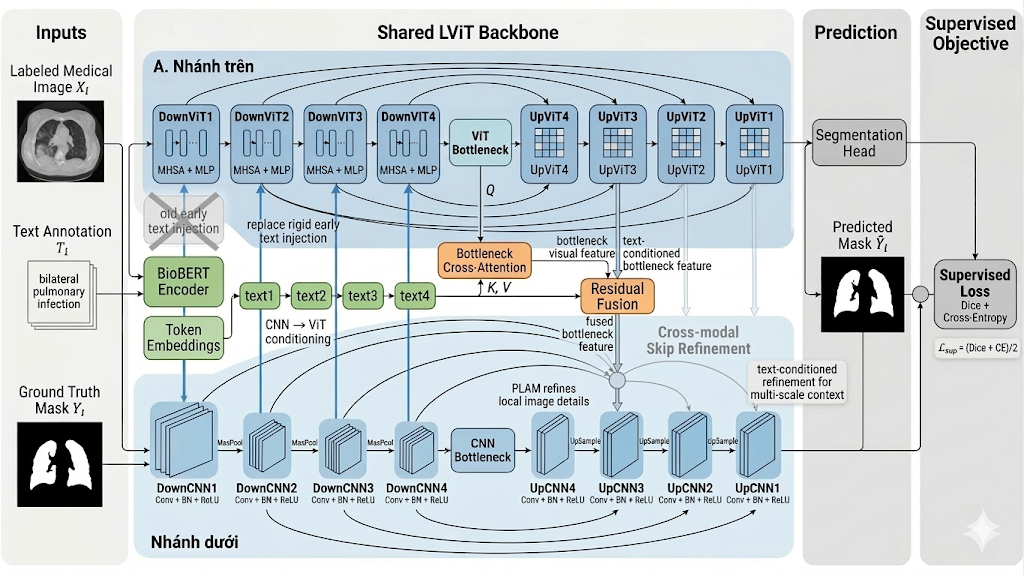
\includegraphics[width=0.9\textwidth,clip,trim=0 18 0 0]{assets/image.png}%
  }{%
    \fbox{\parbox[c][0.28\textheight][c]{0.88\textwidth}{\centering
    Placeholder for the proposed pipeline figure.}}%
  }
  \caption{Pipeline đề xuất cho \texttt{LViTImproved}: ảnh được mã hóa qua encoder, văn bản được chiếu vào cùng không gian đặc trưng, hai nguồn thông tin được hợp nhất tại bottleneck và truyền xuống decoder qua skip connection có điều kiện văn bản.}
  \label{fig:proposed-pipeline}
\end{figure*}

Với cấu hình đã chạy, mô hình có 35,400,433 tham số huấn luyện. Các thành phần cốt lõi gồm stem convolution, bốn tầng downsample, Transformer bottleneck, text conditioner, prototype memory bank, bottleneck cross-attention, text spatial prior, upper-scale fusion tùy chọn, bốn khối upsample-fusion và segmentation head. Đầu ra cuối cùng là logits phân đoạn, được cộng thêm prior logits sinh từ văn bản trước khi tính xác suất.

\subsection{Các cải tiến chính}

\textbf{Bottleneck cross-attention.} Thay vì chỉ nối hoặc cộng đặc trưng văn bản vào ảnh, mô hình tạo một tập bottleneck token học được. Các token này lần lượt attention đến text token và visual token, sau đó truyền thông tin ngược lại cho visual token. Cổng điều khiển \texttt{gate} được tính từ pooled visual và pooled text giúp kiểm soát mức ảnh hưởng của thông tin văn bản, tránh trường hợp văn bản nhiễu chi phối hoàn toàn đặc trưng ảnh.

\textbf{Structured text conditioner.} Thành phần này chiếu text embedding 768 chiều sang không gian bottleneck 512 chiều. Nếu có structured attributes, mô hình cộng thêm attribute context vào text token. Khi văn bản bị thiếu hoặc bị dropout trong training, mô hình dùng fallback token và prototype summary để giảm phụ thuộc tuyệt đối vào text.

\textbf{Text spatial prior.} \texttt{TextSpatialPrior} biến tóm tắt văn bản thành bản đồ prior không gian thô. Mô-đun này dùng các basis map như trung tâm, trái, phải, trên, dưới, dải dọc và dải ngang, sau đó học trọng số từ text summary. Prior này được đưa vào decoder và được chiếu thành \texttt{prior\_logits} để cộng với segmentation logits. Cách thiết kế này phù hợp với QaTa-COV19 vì mô tả văn bản thường chứa thông tin vị trí như \emph{lower left lung}, \emph{all right lung}, hoặc \emph{bilateral pulmonary infection}.

\textbf{Prototype memory bank.} \texttt{PrototypeMemoryBank} lưu các prototype ngữ nghĩa và truy xuất vector thay thế dựa trên visual summary. Trong training, memory được cập nhật bằng momentum từ các mẫu có text hợp lệ. Khi text bị dropout, mô hình vẫn có một summary ngữ nghĩa dự phòng, giúp ổn định huấn luyện và hỗ trợ suy luận trong tình huống thông tin văn bản không đầy đủ.

\textbf{Cross-modal skip refinement.} Decoder không dùng skip feature nguyên bản. Mỗi skip feature được đưa qua \texttt{CrossModalSkipAdapter}, trong đó channel gate lấy từ fused context và spatial gate lấy từ text prior. Nhờ đó, mô hình vẫn giữ lợi thế định vị biên của U-Net nhưng cho phép thông tin văn bản điều chỉnh các skip connection ở nhiều tỉ lệ.

\textbf{Uncertainty-aware pseudo-label fusion.} Với dữ liệu không nhãn, EMA teacher sinh visual pseudo-label, còn text prior cung cấp prior prediction. \texttt{UncertaintyAwarePseudoLabelFusion} chỉ ưu tiên visual pseudo-label khi entropy thấp và độ đồng thuận coarse Dice với text prior vượt ngưỡng. Nếu không, pseudo-label được điều chỉnh theo text prior. Cơ chế này nhằm giảm rủi ro dùng pseudo-label kém tin cậy.

\subsection{Hàm mất mát}

Với dữ liệu có nhãn, mô hình dùng tổng BCE và Dice loss:
\begin{align}
  L_{\mathrm{sup}} = L_{\mathrm{BCE}} + L_{\mathrm{Dice}}.
\end{align}

Với dữ liệu không nhãn, objective gồm consistency loss, text-guidance loss, boundary consistency loss và prototype alignment loss:
\[
\begin{aligned}
  L = L_{\mathrm{sup}}
  + \lambda_{\mathrm{cons}} L_{\mathrm{cons}}
  + \lambda_{\mathrm{text}} L_{\mathrm{text}} \\
  + \lambda_{\mathrm{bd}} L_{\mathrm{boundary}}
  + \lambda_{\mathrm{proto}} L_{\mathrm{proto}}.
\end{aligned}
\]
Trong code hiện tại, các hệ số mặc định là $\lambda_{\mathrm{cons}}=1.0$, $\lambda_{\mathrm{text}}=0.5$, $\lambda_{\mathrm{bd}}=0.25$ và $\lambda_{\mathrm{proto}}=0.1$.

\section{Yêu cầu 3: Thực nghiệm trên QaTa-COV19}

\subsection{Mô tả dữ liệu và insight}

QaTa-COV19 là tập dữ liệu phân đoạn tổn thương COVID-19 trên ảnh X-quang ngực. Dữ liệu phù hợp với mục tiêu của đề tài vì mỗi mẫu gồm ảnh, mask phân đoạn và mô tả văn bản liên quan đến vị trí nhiễm trùng phổi. Theo output chạy thực nghiệm, pipeline sử dụng 5716 mẫu train và 1429 mẫu validation. Ngoài ra, các file text tạm thời trong workspace cho thấy file \texttt{Test\_text.xlsx} có 2113 mẫu mô tả văn bản, nhưng script huấn luyện hiện tại chưa dùng \texttt{Test\_Folder} để đánh giá test.

Các mô tả văn bản có cấu trúc khá ngắn và giàu thông tin vị trí. Trong \texttt{Train\_text.xlsx}, trung bình mỗi mô tả dài khoảng 84.4 ký tự hoặc 12.4 từ, có 301 mô tả duy nhất trên 7145 dòng. Khoảng 79.3\% mô tả chứa từ \emph{Bilateral}, 36.6\% chứa \emph{all left lung}, và 32.0\% chứa \emph{all right lung}. Năm mô tả phổ biến nhất đều xoay quanh nhiễm trùng hai bên hoặc vùng lower lung. Điều này giải thích vì sao text spatial prior là một cải tiến hợp lý: văn bản không chỉ mô tả bệnh có/không, mà còn cung cấp tín hiệu định vị tương đối trong phổi.

\begin{figure*}[t]
  \centering
  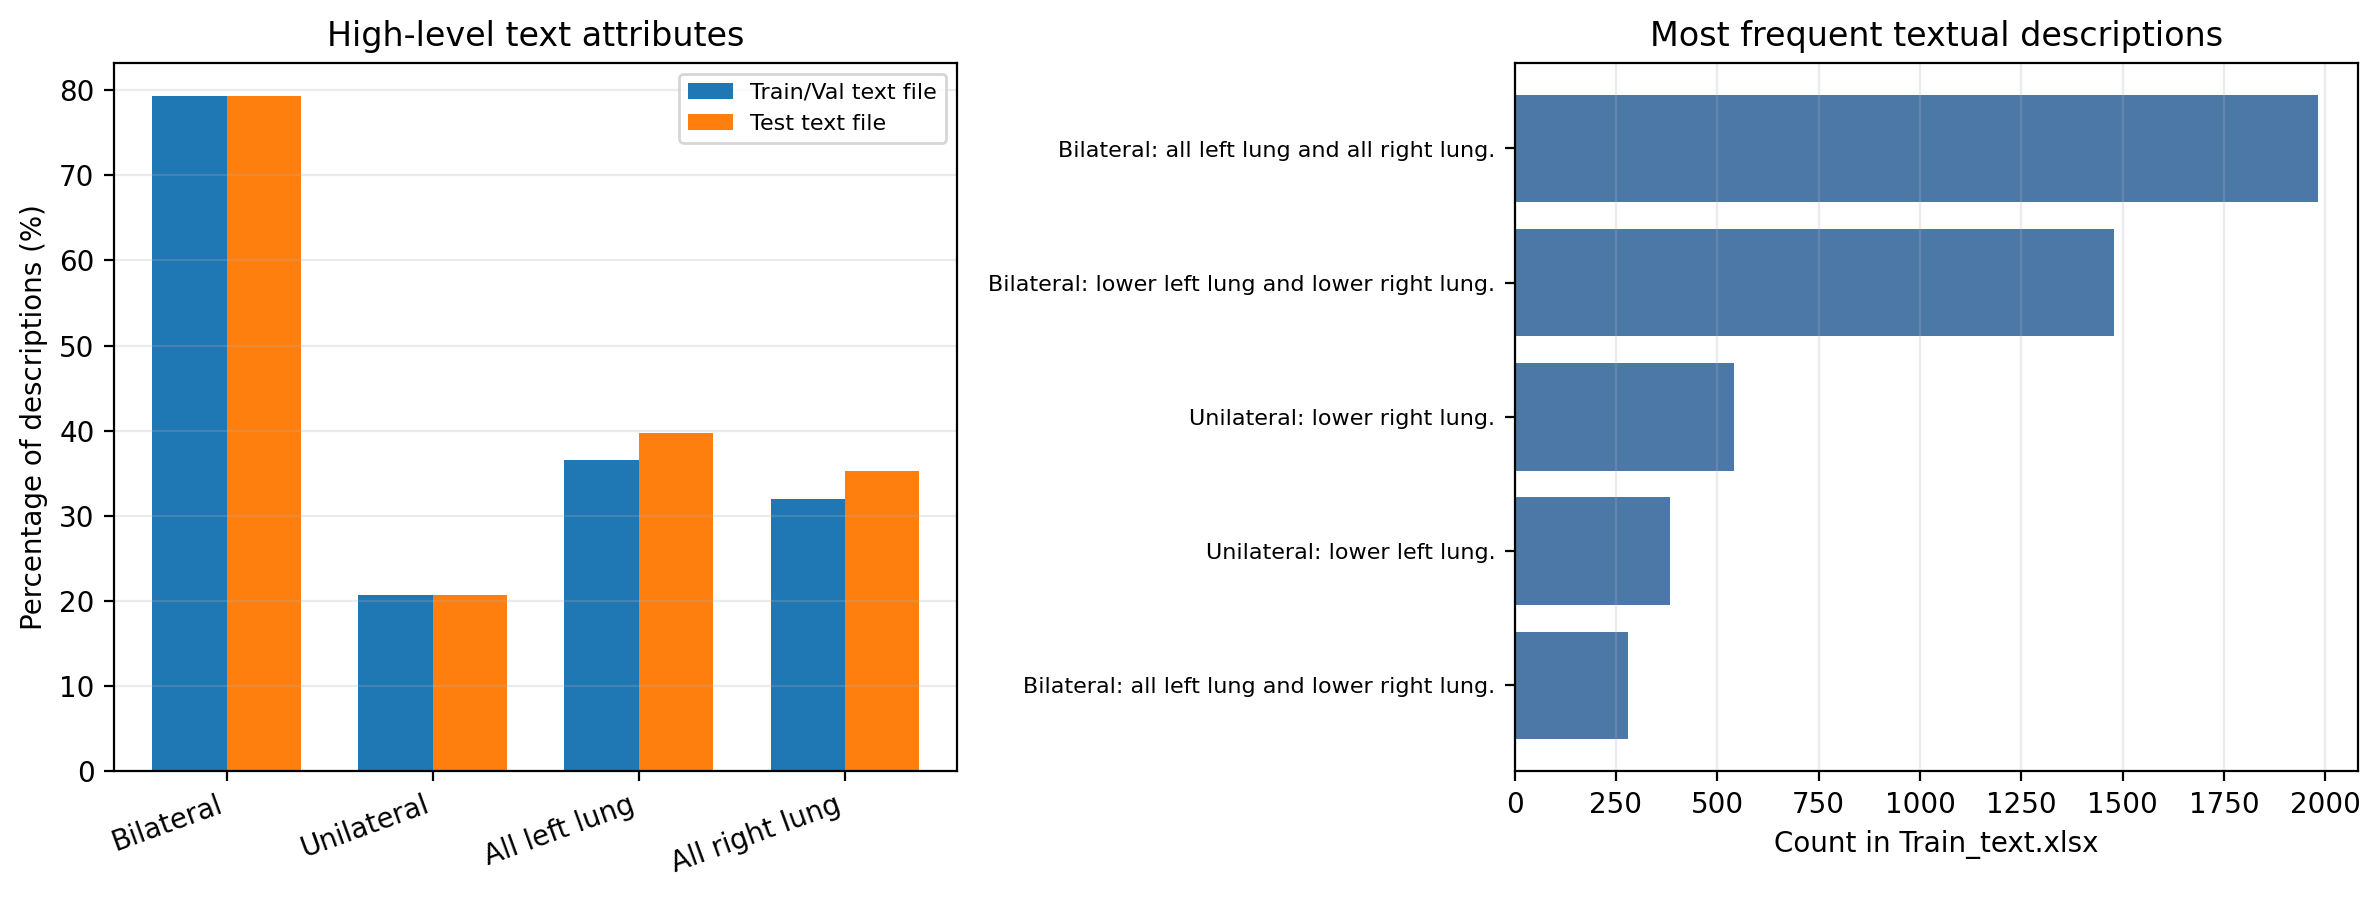
\includegraphics[width=0.96\textwidth]{figures/qatacov19_text_insights.png}
  \caption{Insight từ mô tả văn bản của QaTa-COV19: phần lớn mô tả là bilateral và chứa chỉ dẫn vùng phổi, tạo cơ sở cho text spatial prior trong \texttt{LViTImproved}.}
  \label{fig:qatacov19-text-insights}
\end{figure*}

Một điểm cần lưu ý là phân bố mô tả không cân bằng. Mô tả ``Bilateral pulmonary infection, two infected areas, all left lung and all right lung'' xuất hiện 1981 lần trong file train text, còn mô tả ``Bilateral pulmonary infection, two infected areas, lower left lung and lower right lung'' xuất hiện 1478 lần. Vì vậy, text branch có thể học được prior mạnh cho một số mẫu phổ biến, nhưng cũng có nguy cơ kém linh hoạt với ca hiếm hơn. Đây là lý do cần phân tích định tính sau khi có prediction trên validation hoặc test.

\subsection{Thiết lập thực nghiệm}

Hai output Kaggle được dùng trong báo cáo là \texttt{tqc0103/lvit-improved-qatacovid19-1-0} cho thiết lập 100\% nhãn và \texttt{tqc0103/lvit-improved-qatacovid19-0-5} cho thiết lập 50\% nhãn. Mỗi output có 501 file, bao gồm checkpoint, history, cấu hình chạy, summary và kernel log. Output 100\% nhãn có dung lượng khoảng 7.41GB vì lưu nhiều checkpoint trung gian; output 50\% nhãn có dung lượng khoảng 1.07GB.

\begin{table}[t]
  \centering
  \caption{Cấu hình chung của hai run trên QaTa-COV19.}
  \label{tab:run-config}
  \scriptsize
  \begin{tabularx}{\columnwidth}{lX}
    \toprule
    Hạng mục & Giá trị \\
    \midrule
    Epoch & 120 \\
    Batch size & 12 \\
    Gradient accumulation & 4 bước \\
    Effective batch size & 48 \\
    Optimizer & AdamW \\
    Learning rate & $10^{-4}$ \\
    Minimum learning rate & $10^{-6}$ \\
    Weight decay & $10^{-4}$ \\
    Scheduler & Cosine annealing \\
    EMA decay & 0.99 \\
    Device & CUDA \\
    AMP & Tắt \\
    Text encoder & BiomedBERT base uncased abstract fulltext \\
    Trainable parameters & 35,400,433 \\
    \bottomrule
  \end{tabularx}
\end{table}

Thiết lập 100\% nhãn sử dụng toàn bộ 5716 mẫu train làm labeled set, không có unlabeled set. Thiết lập 50\% nhãn chia 5716 mẫu train thành 2858 mẫu labeled và 2858 mẫu unlabeled với seed 666. Cả hai thiết lập đều đánh giá trên 1429 mẫu validation.

\begin{table}[t]
  \centering
  \caption{Số lượng mẫu trong hai thiết lập.}
  \label{tab:data-split}
  \scriptsize
  \begin{tabular}{lccc}
    \toprule
    Thiết lập & Labeled & Unlabeled & Validation \\
    \midrule
    100\% nhãn & 5716 & 0 & 1429 \\
    50\% nhãn & 2858 & 2858 & 1429 \\
    \bottomrule
  \end{tabular}
\end{table}

\subsection{Kết quả validation}

\begin{table}[t]
  \centering
  \caption{Kết quả validation của \texttt{LViTImproved}.}
  \label{tab:qatacov19-results}
  \scriptsize
  \begin{tabularx}{\columnwidth}{lccc}
    \toprule
    Thiết lập & Best epoch & Best val Dice & Val Dice epoch 120 \\
    \midrule
    100\% nhãn & 77 & 0.8249 & 0.8222 \\
    50\% nhãn & 60 & 0.7685 & 0.6555 \\
    \bottomrule
  \end{tabularx}
\end{table}

Bảng \ref{tab:qatacov19-results} cho thấy thiết lập 100\% nhãn đạt best validation Dice 0.8249 tại epoch 77. Đến epoch 120, Dice vẫn là 0.8222, chỉ thấp hơn best checkpoint khoảng 0.0027. Điều này cho thấy khi có đầy đủ mask thật, \texttt{LViTImproved} hội tụ tương đối ổn định và không bị suy giảm đáng kể ở cuối training.

Thiết lập 50\% nhãn đạt best validation Dice 0.7685 tại epoch 60, thấp hơn thiết lập 100\% nhãn 0.0564 Dice. Mức giảm này phản ánh ảnh hưởng của việc giảm một nửa số mask thật, nhưng cũng cho thấy mô hình vẫn học được biểu diễn hữu ích khi kết hợp 2858 mẫu có nhãn với 2858 mẫu không nhãn. Tuy nhiên, đến epoch 120, Dice giảm còn 0.6555, thấp hơn best checkpoint 0.1130 Dice. Do đó checkpoint epoch 60 mới là checkpoint nên dùng cho đánh giá tiếp theo ở thiết lập 50\% nhãn.

\begin{table}[t]
  \centering
  \caption{Diễn biến Dice validation tại các epoch tiêu biểu.}
  \label{tab:epoch-progression}
  \scriptsize
  \begin{tabularx}{\columnwidth}{lrrrr}
    \toprule
    Thiết lập & E1 & E20 & E60 & E120 \\
    \midrule
    100\% nhãn & 0.5803 & 0.8049 & 0.8193 & 0.8222 \\
    50\% nhãn & 0.2103 & 0.4627 & 0.7685 & 0.6555 \\
    \bottomrule
  \end{tabularx}
\end{table}

\begin{figure*}[t]
  \centering
  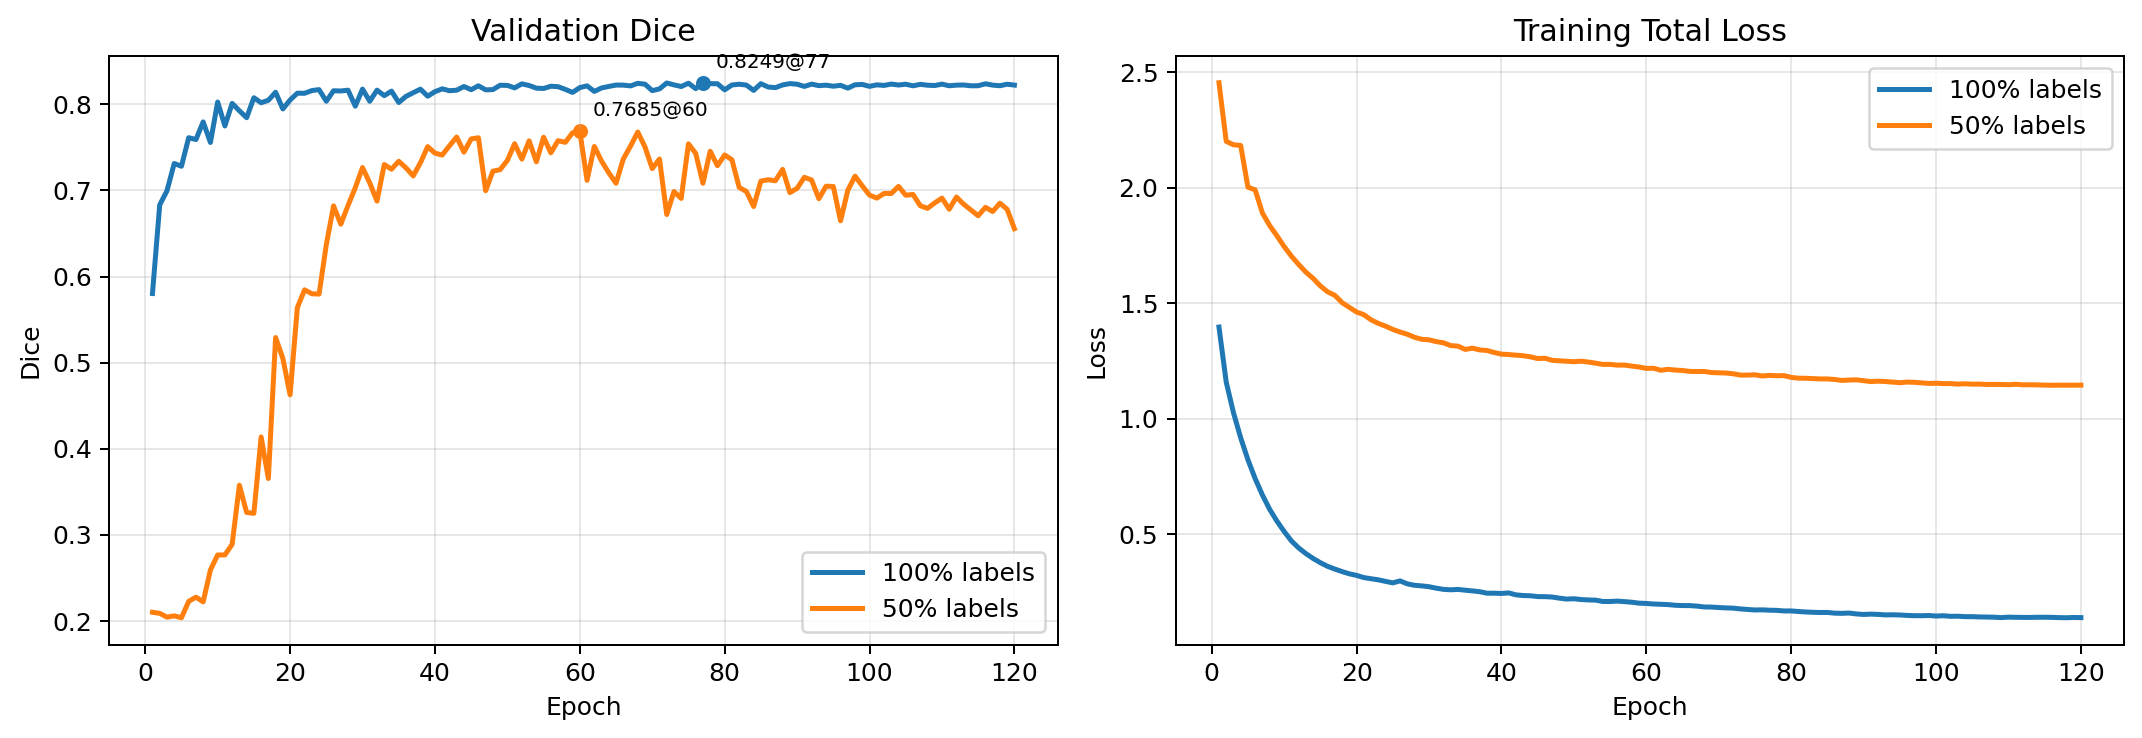
\includegraphics[width=0.95\textwidth]{figures/qatacov19_training_curves.png}
  \caption{Đường cong huấn luyện trên QaTa-COV19. Thiết lập 100\% nhãn hội tụ nhanh và ổn định quanh Dice 0.82; thiết lập 50\% nhãn đạt đỉnh tại epoch 60 rồi giảm dần dù training loss tiếp tục giảm.}
  \label{fig:qatacov19-training-curves}
\end{figure*}

\subsection{Phân tích quá trình huấn luyện}

Ở thiết lập 100\% nhãn, Dice tăng nhanh từ 0.5803 tại epoch 1 lên 0.8025 tại epoch 10. Sau đó mô hình tiếp tục cải thiện chậm hơn, đạt 0.8193 tại epoch 60 và 0.8249 tại epoch 77. Training supervised loss giảm từ 1.3945 xuống 0.1384 ở epoch 120. Vì không có unlabeled set, consistency loss, text-guidance loss và boundary loss đều bằng 0; quá trình tối ưu chủ yếu do supervised BCE--Dice loss điều khiển. Đây là đường cong tương đối tốt cho báo cáo validation vì khoảng cách giữa best epoch và last epoch rất nhỏ.

Ở thiết lập 50\% nhãn, Dice khởi đầu thấp hơn nhiều: 0.2103 tại epoch 1 và 0.2768 tại epoch 10. Từ epoch 20 đến epoch 60, Dice tăng mạnh từ 0.4627 lên 0.7685, cho thấy sau khi supervised branch học được biểu diễn ban đầu, dữ liệu không nhãn và text-guidance bắt đầu hỗ trợ quá trình học. Tuy nhiên, sau epoch 60, Dice giảm dần còn 0.7082 tại epoch 77, 0.6945 tại epoch 100 và 0.6555 tại epoch 120.

Điểm đáng chú ý là ở thiết lập 50\% nhãn, training total loss vẫn giảm từ 1.2175 tại epoch 60 xuống 1.1451 tại epoch 120, trong khi validation Dice giảm. Training supervised loss cũng giảm từ 0.2366 xuống 0.1574. Ngược lại, consistency và text-guidance loss duy trì quanh 0.65. Điều này gợi ý rằng objective bán giám sát ở giai đoạn cuối chưa hoàn toàn tương ứng với chất lượng validation. Một diễn giải hợp lý là pseudo-label hoặc text prior có thể trở nên quá mạnh so với tín hiệu mask thật, khiến student tối ưu tốt hơn trên training objective nhưng không cải thiện trên validation.

\subsection{Giới hạn hiện tại: chưa có test metric}

Hai output Kaggle hiện chỉ chứa \texttt{val\_dice} và \texttt{best\_val\_dice}. Trong \texttt{train\_improved\_ssl.py}, hàm \texttt{build\_datasets} chỉ đọc \texttt{Train\_Folder/Train\_text.xlsx} và \texttt{Val\_Folder/Val\_text.xlsx}; hàm \texttt{validate} được gọi trên validation loader sau mỗi epoch. Chưa có phần đọc \texttt{Test\_Folder}, chưa có vòng lặp test, chưa log test Dice và cũng chưa log mIoU.

Vì vậy, báo cáo hiện tại chỉ kết luận được rằng checkpoint 100\% nhãn có validation Dice tốt nhất 0.8249 và checkpoint 50\% nhãn có validation Dice tốt nhất 0.7685. Để hoàn thiện đánh giá cuối cùng, cần chạy thêm test evaluation trên \texttt{best\_model.pt} của từng thiết lập. Bước test nên lưu tối thiểu test Dice, test mIoU, mean precision/recall nếu cần, và một số ảnh minh họa gồm ảnh gốc, mask thật, prediction và overlay lỗi.

\section{Thảo luận}

Kết quả cho thấy \texttt{LViTImproved} hoạt động ổn định hơn khi có đầy đủ nhãn. Điều này phù hợp với trực giác vì supervised mask là tín hiệu trực tiếp nhất cho phân đoạn. Trong thiết lập 100\%, các mô-đun ảnh--văn bản vẫn có thể hỗ trợ biểu diễn, nhưng quá trình học không phải phụ thuộc vào pseudo-label.

Thiết lập 50\% nhãn là phần quan trọng hơn cho mục tiêu cải tiến. Best validation Dice 0.7685 cho thấy mô hình không sụp đổ khi chỉ dùng một nửa số mask thật. Tuy nhiên, sự suy giảm sau epoch 60 cho thấy pipeline bán giám sát cần được điều chỉnh. Các hướng cải thiện hợp lý gồm early stopping theo validation Dice, giảm dần $\lambda_{\mathrm{cons}}$ hoặc $\lambda_{\mathrm{text}}$ sau khi validation Dice đạt đỉnh, tăng ngưỡng confidence trong pseudo-label fusion, và kiểm tra định tính các prediction giai đoạn cuối để xem mô hình đang over-segment hay under-segment vùng tổn thương.

Về dataset, insight văn bản cho thấy QaTa-COV19 có mô tả vị trí khá rõ, đặc biệt là các cụm từ liên quan đến bilateral, lower lung, all left lung và all right lung. Điều này ủng hộ thiết kế text spatial prior. Tuy nhiên, phân bố mô tả cũng tập trung mạnh vào một số câu phổ biến, nên cần cẩn thận với nguy cơ mô hình học prior quá chung. Nếu có thêm thời gian, nên phân nhóm validation theo loại mô tả, ví dụ bilateral so với unilateral, lower lung so với all lung, để xem mô hình cải thiện hoặc suy giảm ở nhóm nào.

Giới hạn lớn nhất của báo cáo hiện tại là thiếu test metric và thiếu baseline chạy cùng cấu hình. Kết quả validation đủ để chứng minh nhóm đã thực nghiệm mô hình đề xuất trên một tập dữ liệu chuẩn, nhưng chưa đủ để khẳng định mô hình vượt U-Net, LViT gốc hoặc các ablation khác. Bước tiếp theo nên chạy test cho best checkpoint, thêm baseline U-Net/LViT gốc, và chạy ablation bỏ từng mô-đun: text spatial prior, bottleneck cross-attention, prototype memory bank và cross-modal skip adapter.

\section{Kết luận}

Báo cáo đã trình bày mô hình \texttt{LViTImproved} theo \textbf{Yêu cầu 2} và thực nghiệm trên QaTa-COV19 theo \textbf{Yêu cầu 3}. Về mô hình, cải tiến chính nằm ở việc kết hợp encoder--decoder, Transformer bottleneck, bottleneck cross-attention, text spatial prior, prototype memory bank, cross-modal skip refinement và học bán giám sát dựa trên EMA teacher. Về thực nghiệm, hai run Kaggle đã hoàn tất ở thiết lập 100\% và 50\% nhãn. Best validation Dice lần lượt là 0.8249 tại epoch 77 và 0.7685 tại epoch 60. Kết quả này cho thấy mô hình có khả năng học phân đoạn trên QaTa-COV19 và vẫn giữ năng lực tương đối tốt khi giảm một nửa số mask thật. Tuy nhiên, vì chưa có test evaluation, kết luận cuối cùng cần được bổ sung bằng đánh giá test set độc lập, mIoU, baseline và ablation study.

% !TeX root = ../main.tex
